\section{Resumo}


\begin{figure}[h!]
    \centering
    \label{fig1}
    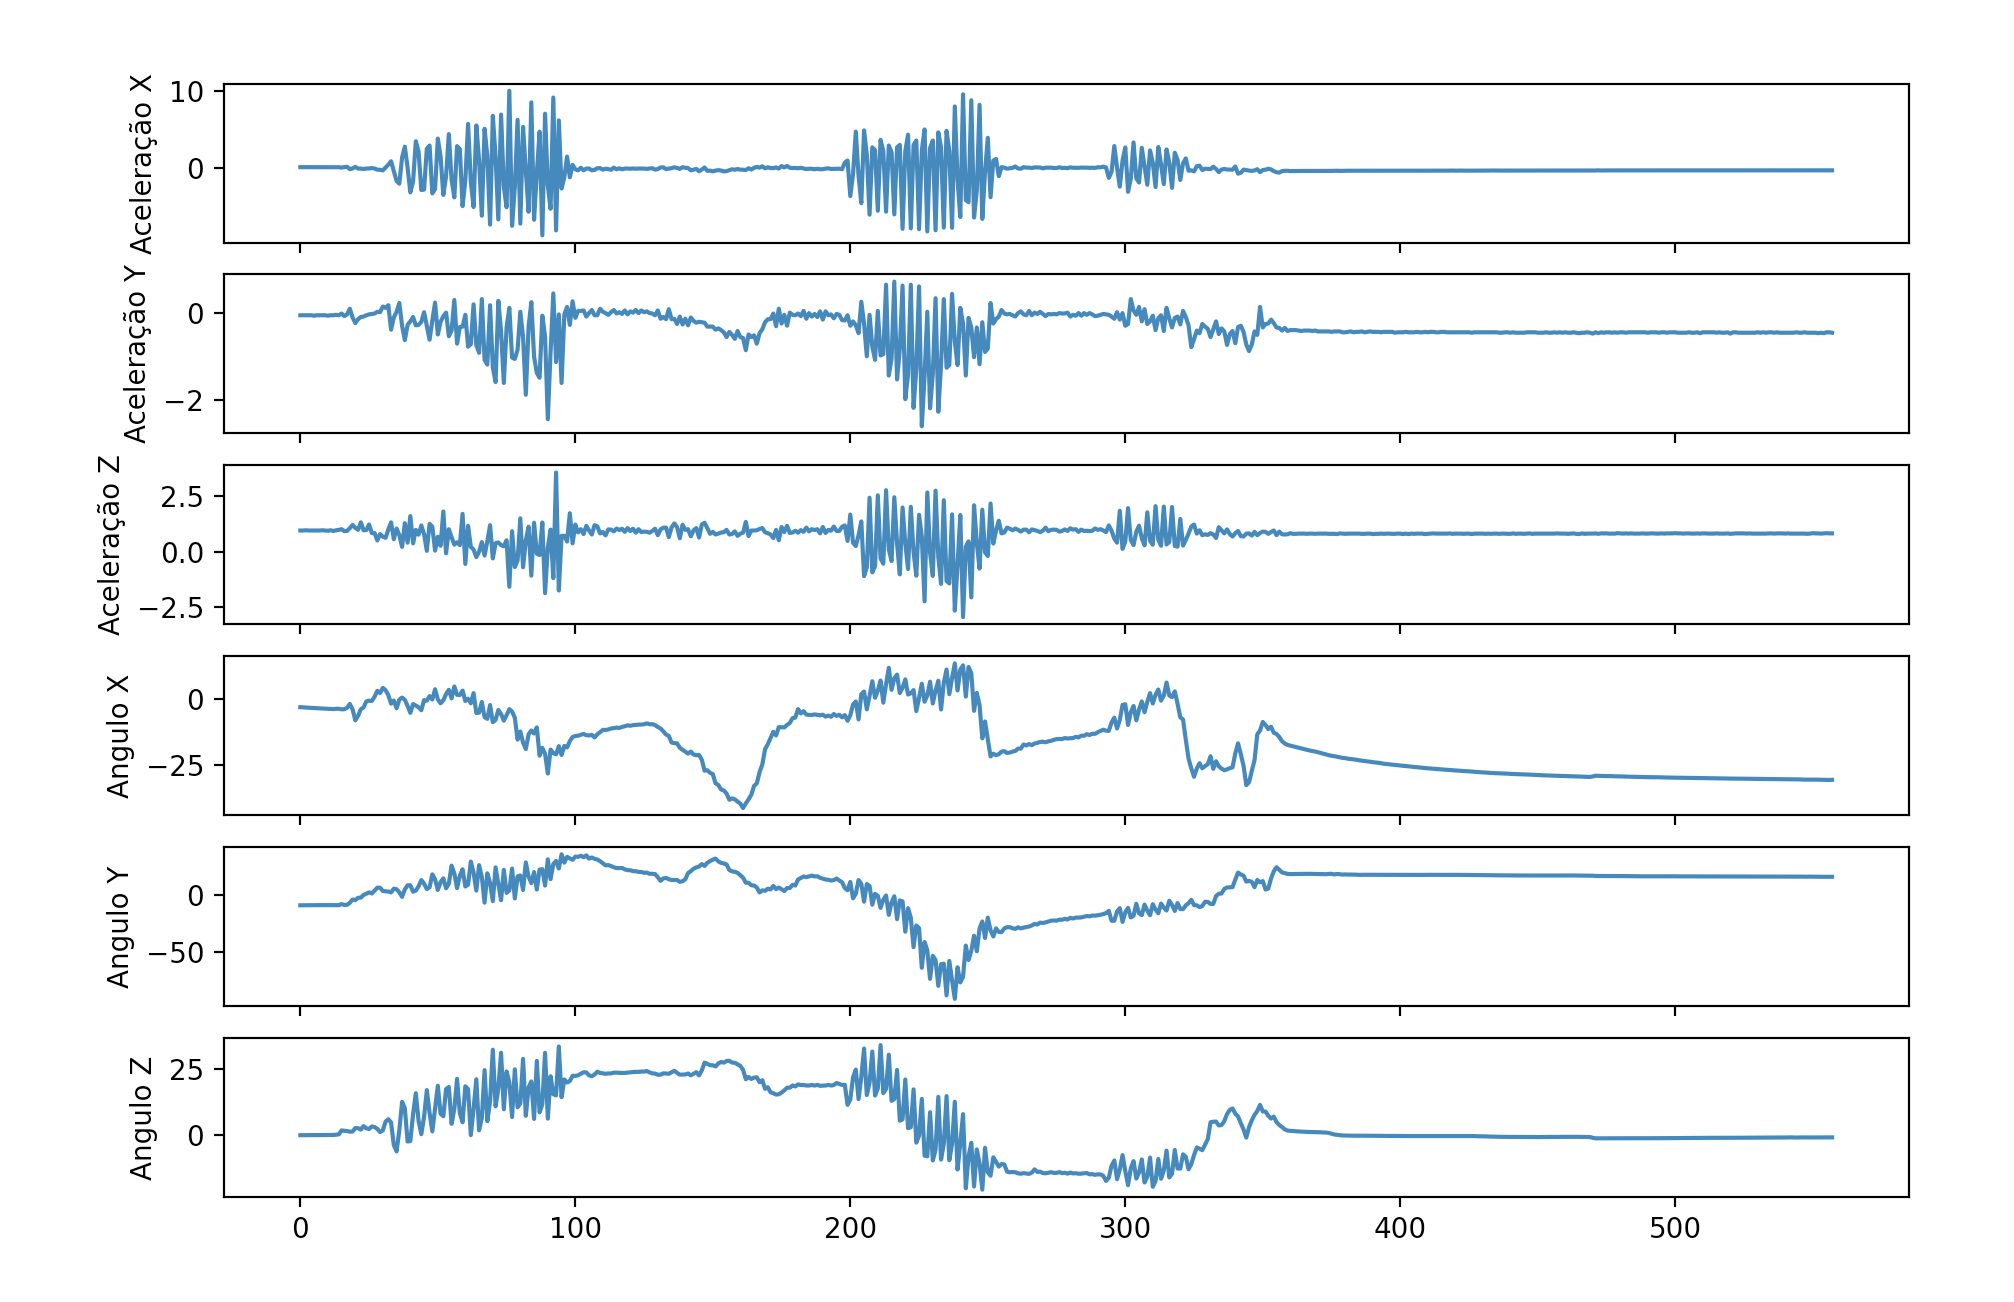
\includegraphics[scale=0.2]{images/VibracaoX.png}
    \caption{VibracaoX}
\end{figure}

\begin{figure}[h!]
    \centering
    \label{fig2}
    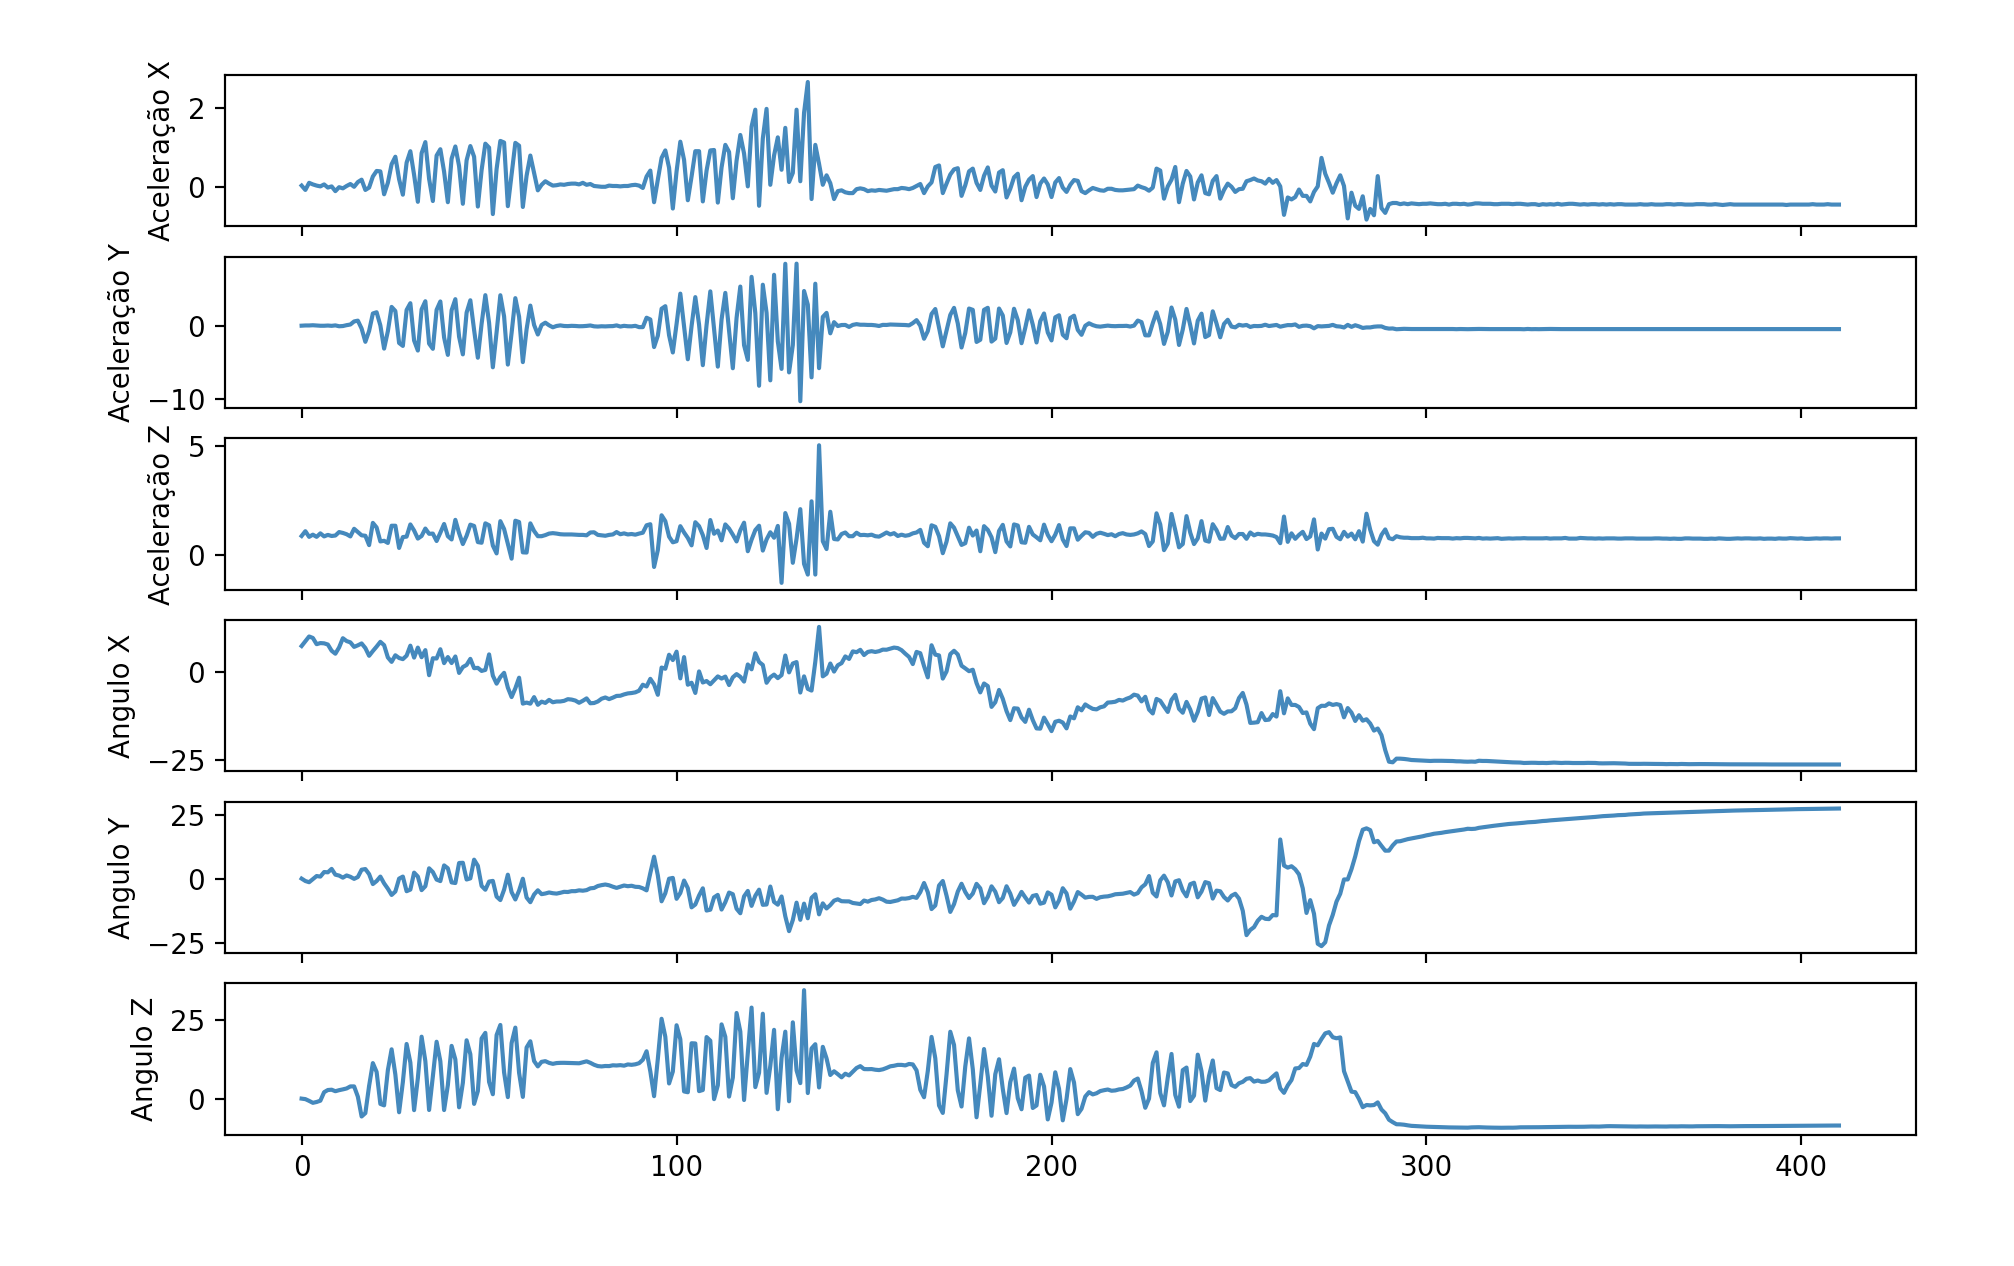
\includegraphics[scale=0.2]{images/VibracaoY.png}
    \caption{VibracaoY}
\end{figure}

\begin{figure}[h!]
    \centering
    \label{fig3}
    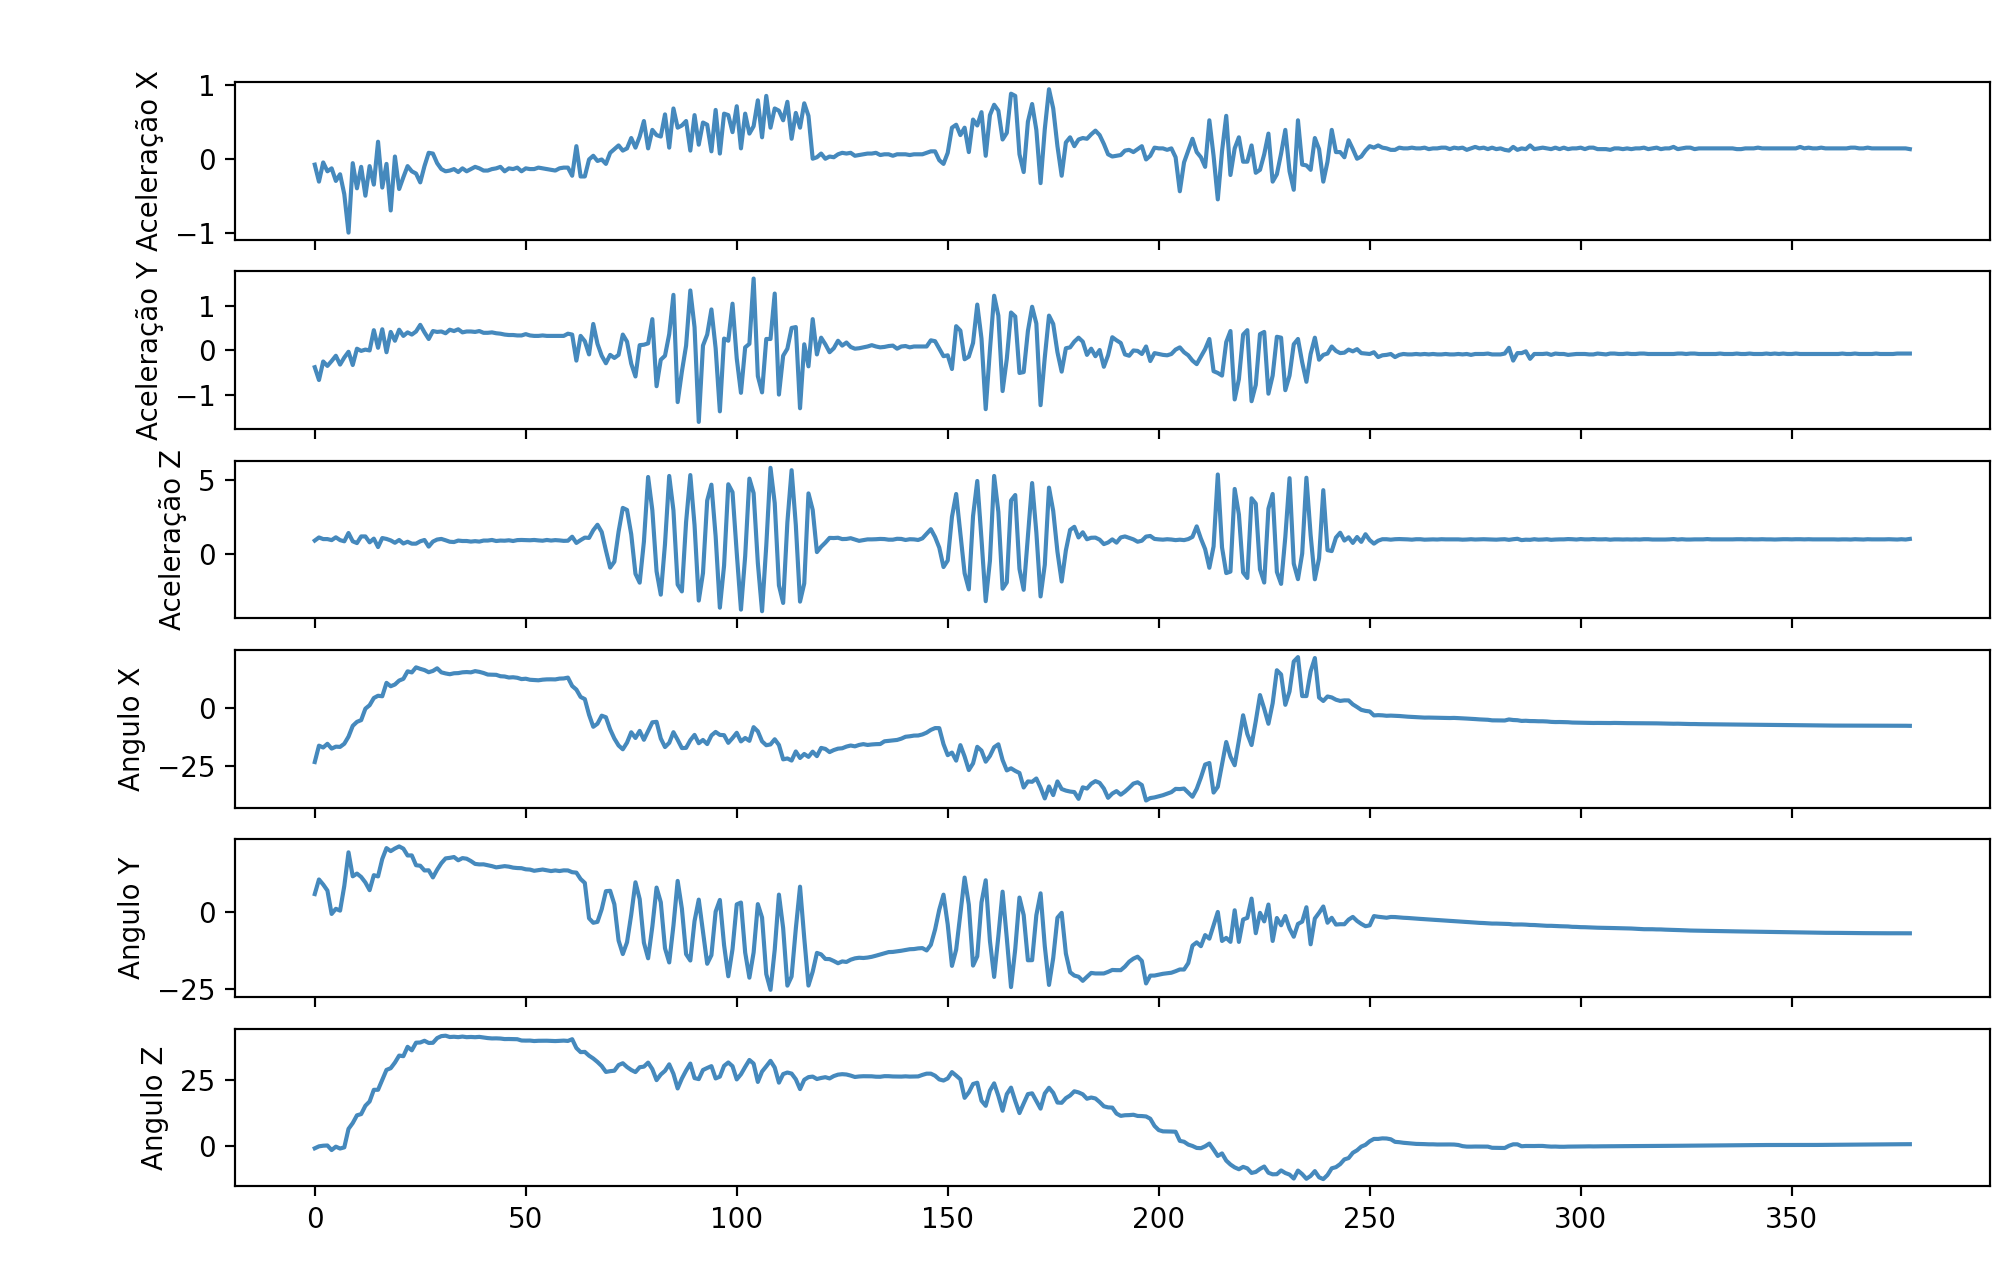
\includegraphics[scale=0.2]{images/VibracaoZ.png}
    \caption{VibracaoZ}
\end{figure}

\begin{figure}[h!]
    \centering
    \label{fig4}
    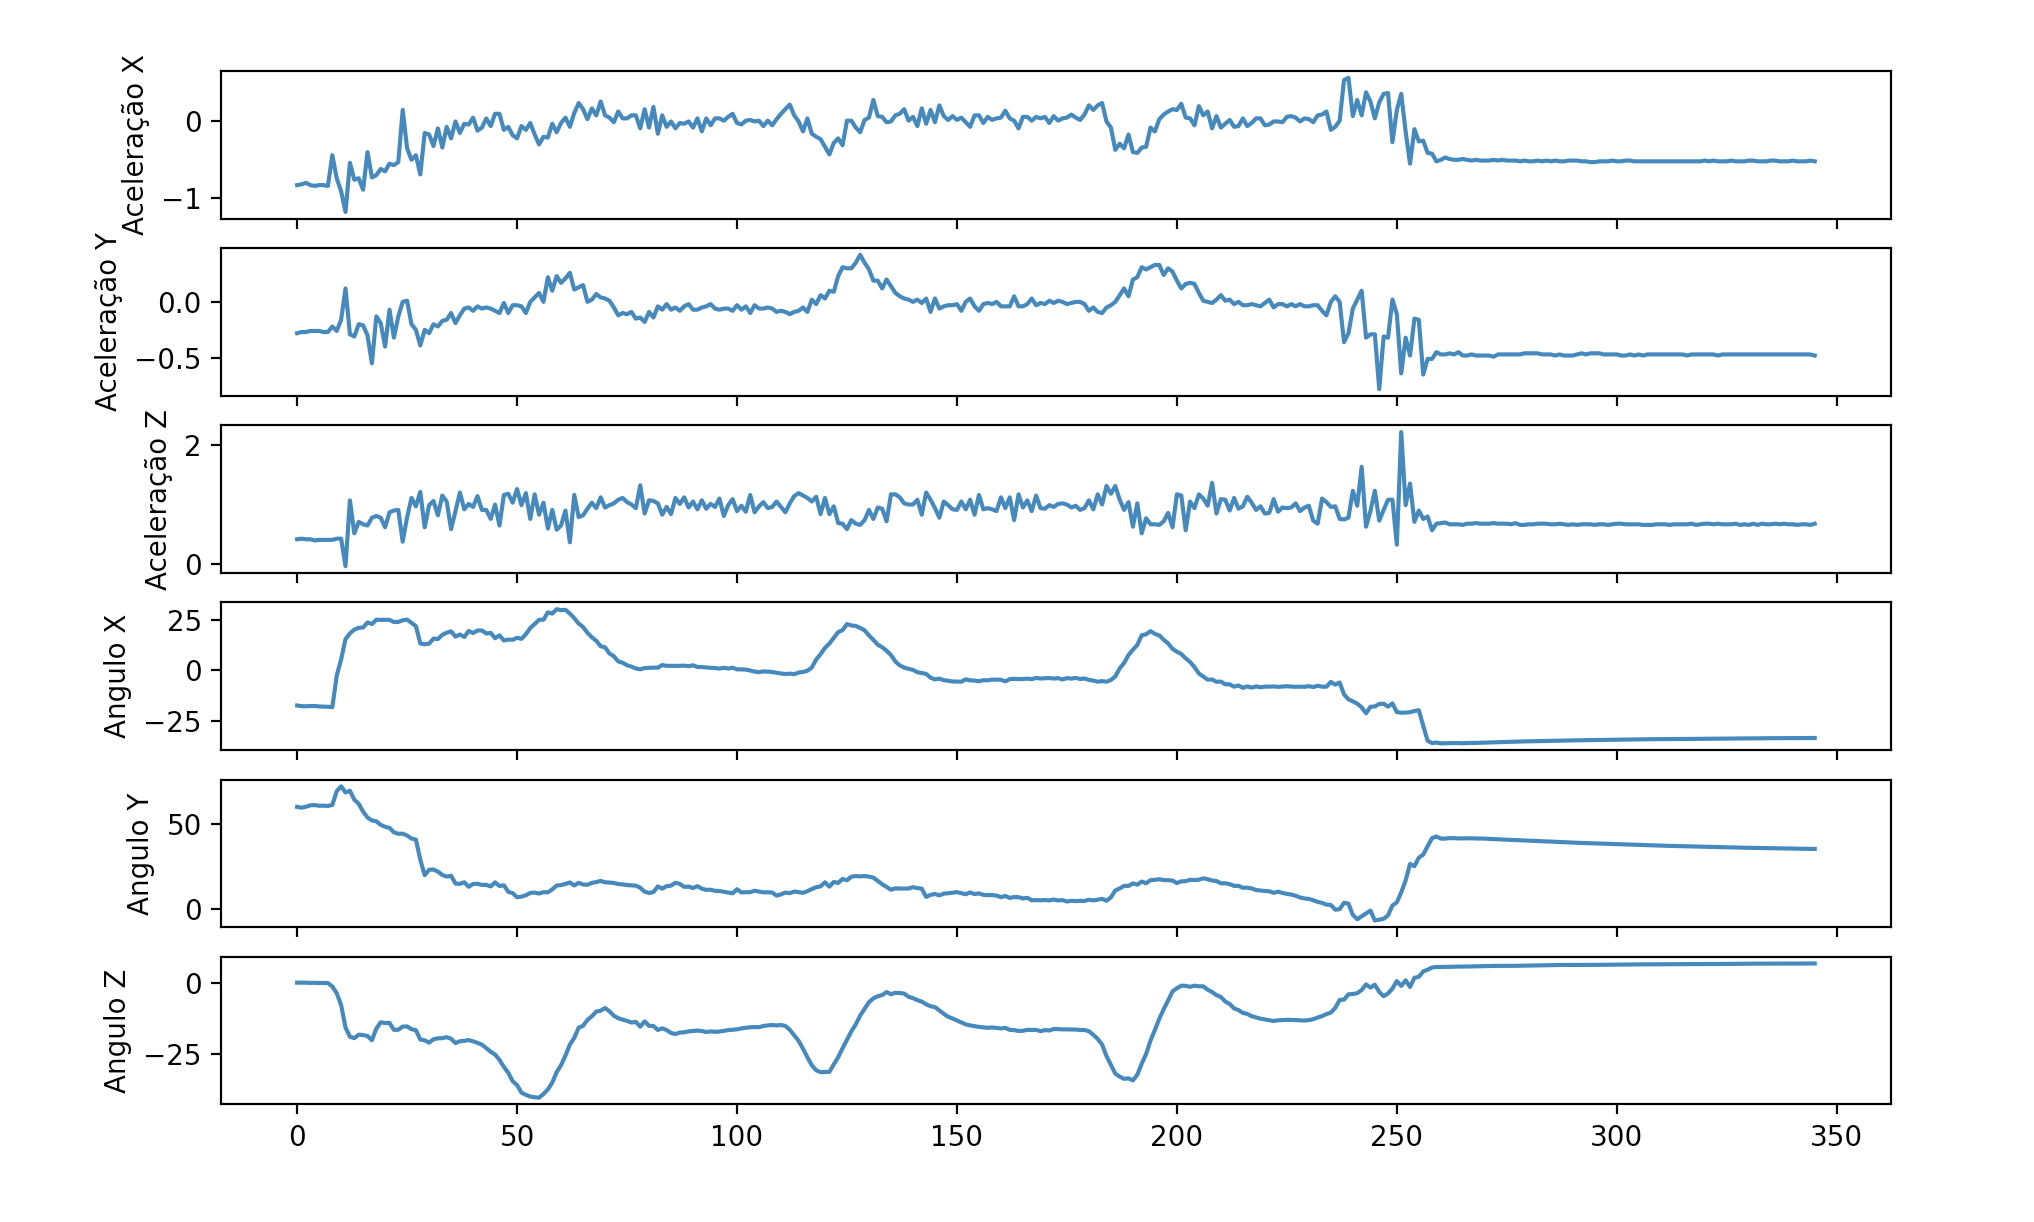
\includegraphics[scale=0.2]{images/CirculoZ.png}
    \caption{CirculoZ}
\end{figure}
\begin{figure}[h!]
    \centering
    \label{fig5}
    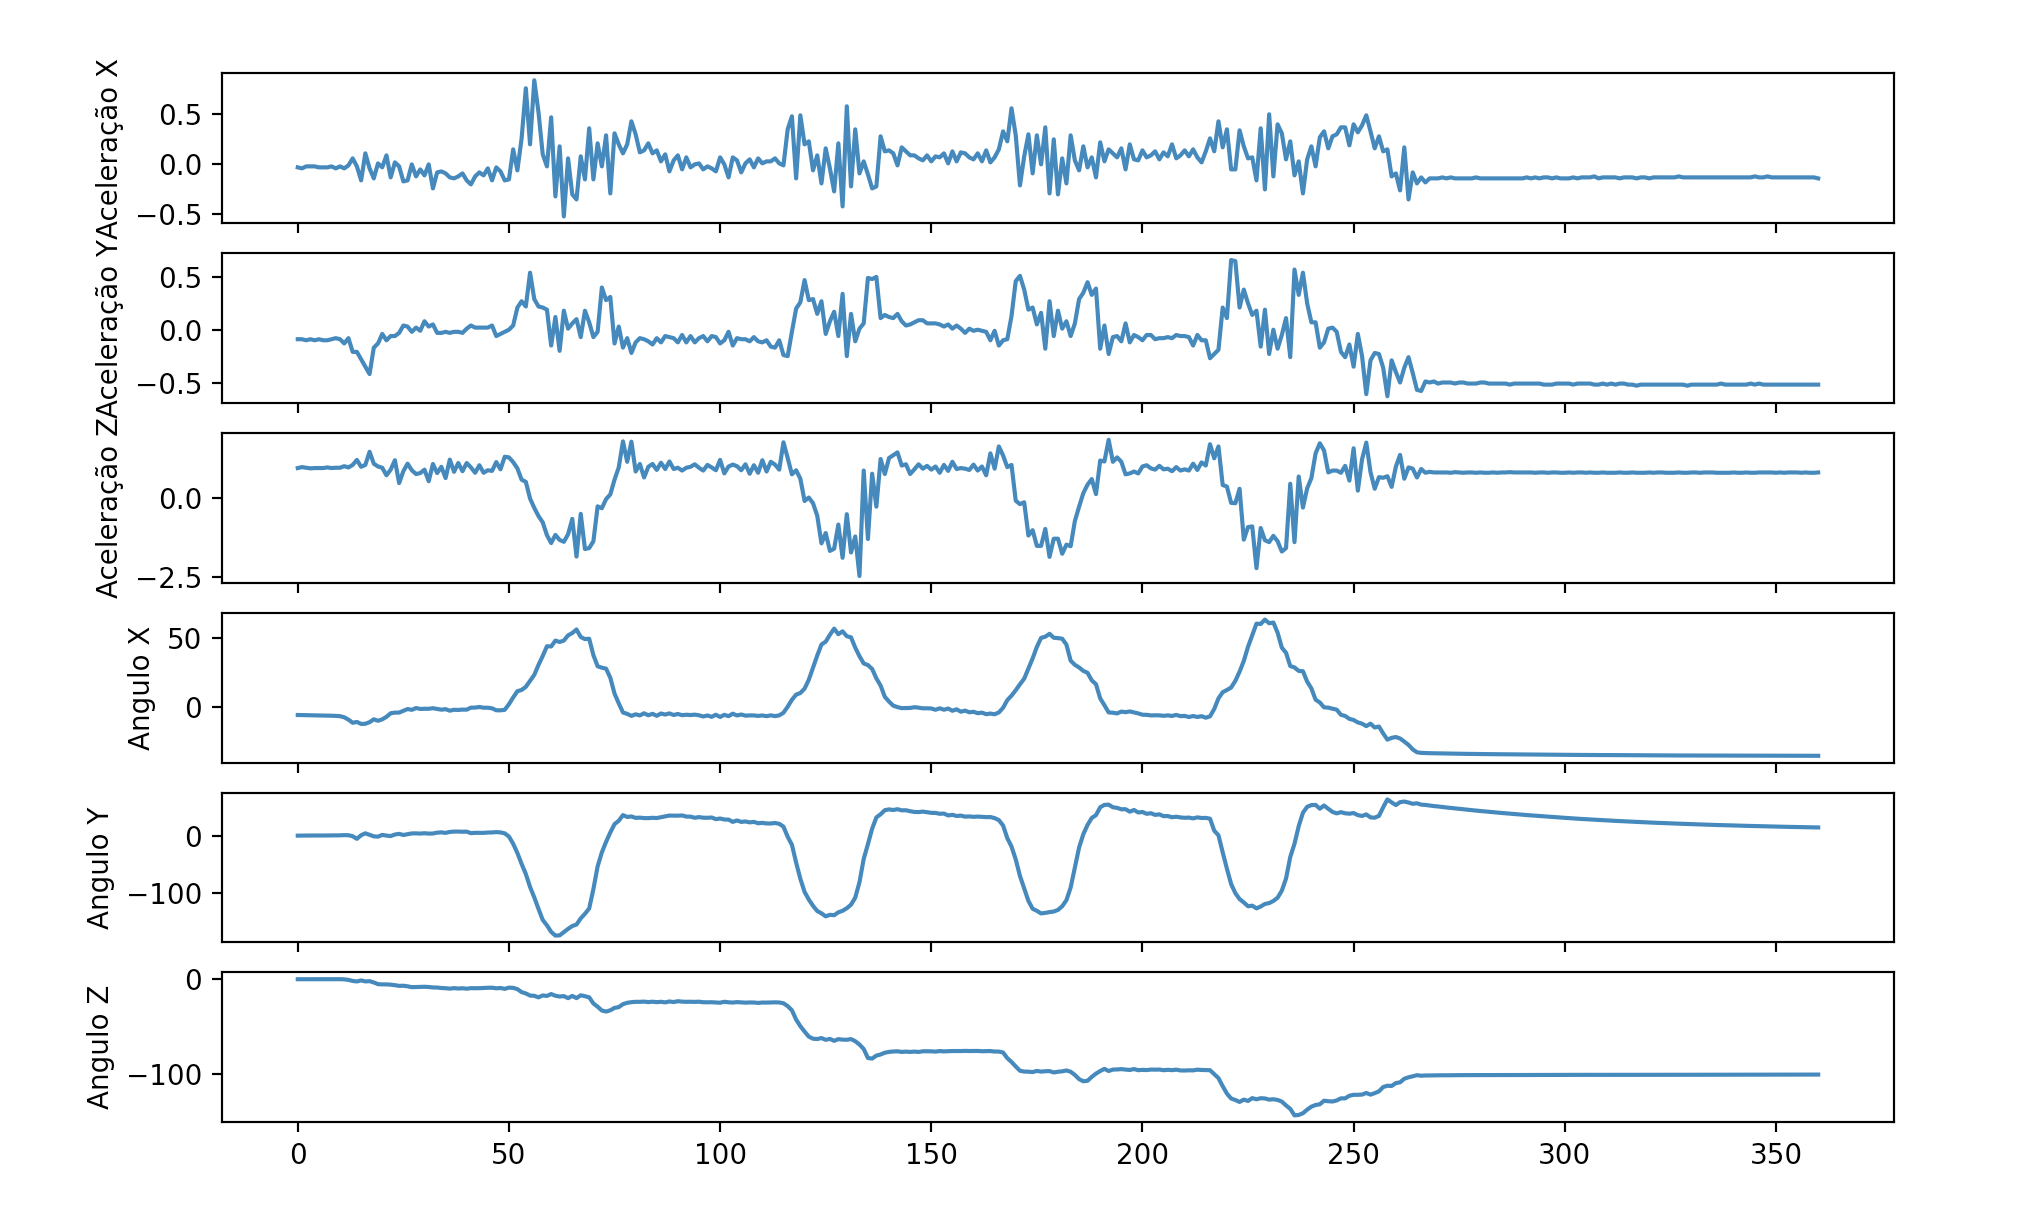
\includegraphics[scale=0.2]{images/GiraeVoltaY.png}
    \caption{GiraeVoltaY}
\end{figure}
